\subsubsection{Which implementation technologies and tools are adopted by software development professionals?}
\label{tools}

Our survey included five questions to find technologies and tools that are adopted by software development professionals. To answer this question fully, we report the following results:

\begin{itemize}
\item Technology Platform (Q 9).
\item Operating System (Q 10).
\item Programming Language (Q 11).
\item Framework (Q 12).
\item IDE (Q 13).
\end{itemize}


\paragraph{Technology Platforms}
Participants were allowed to choose multiple options. As shown in Figure \ref{fig:platforms}, most of our survey respondents (80\%) work in web platform. The rests are mobile (45\%), Desktop (30\%), Embedded/IOT (8\%). This result shows that clients of software products heavily rely on web-based services. We have conducted a cross aspect analysis to identify any relationship between the technology platform and the requirement gathering process. The bubble charts in Figure \ref{fig:requirement technology cross analysis} visualize the cross-aspect analysis. It is clear from Figure \ref{fig:requirement technology cross analysis} that the requirement gathering process is mostly practiced in GUI based development (e.g., web, desktop, mobile).

\begin{figure}[h]
\centering
  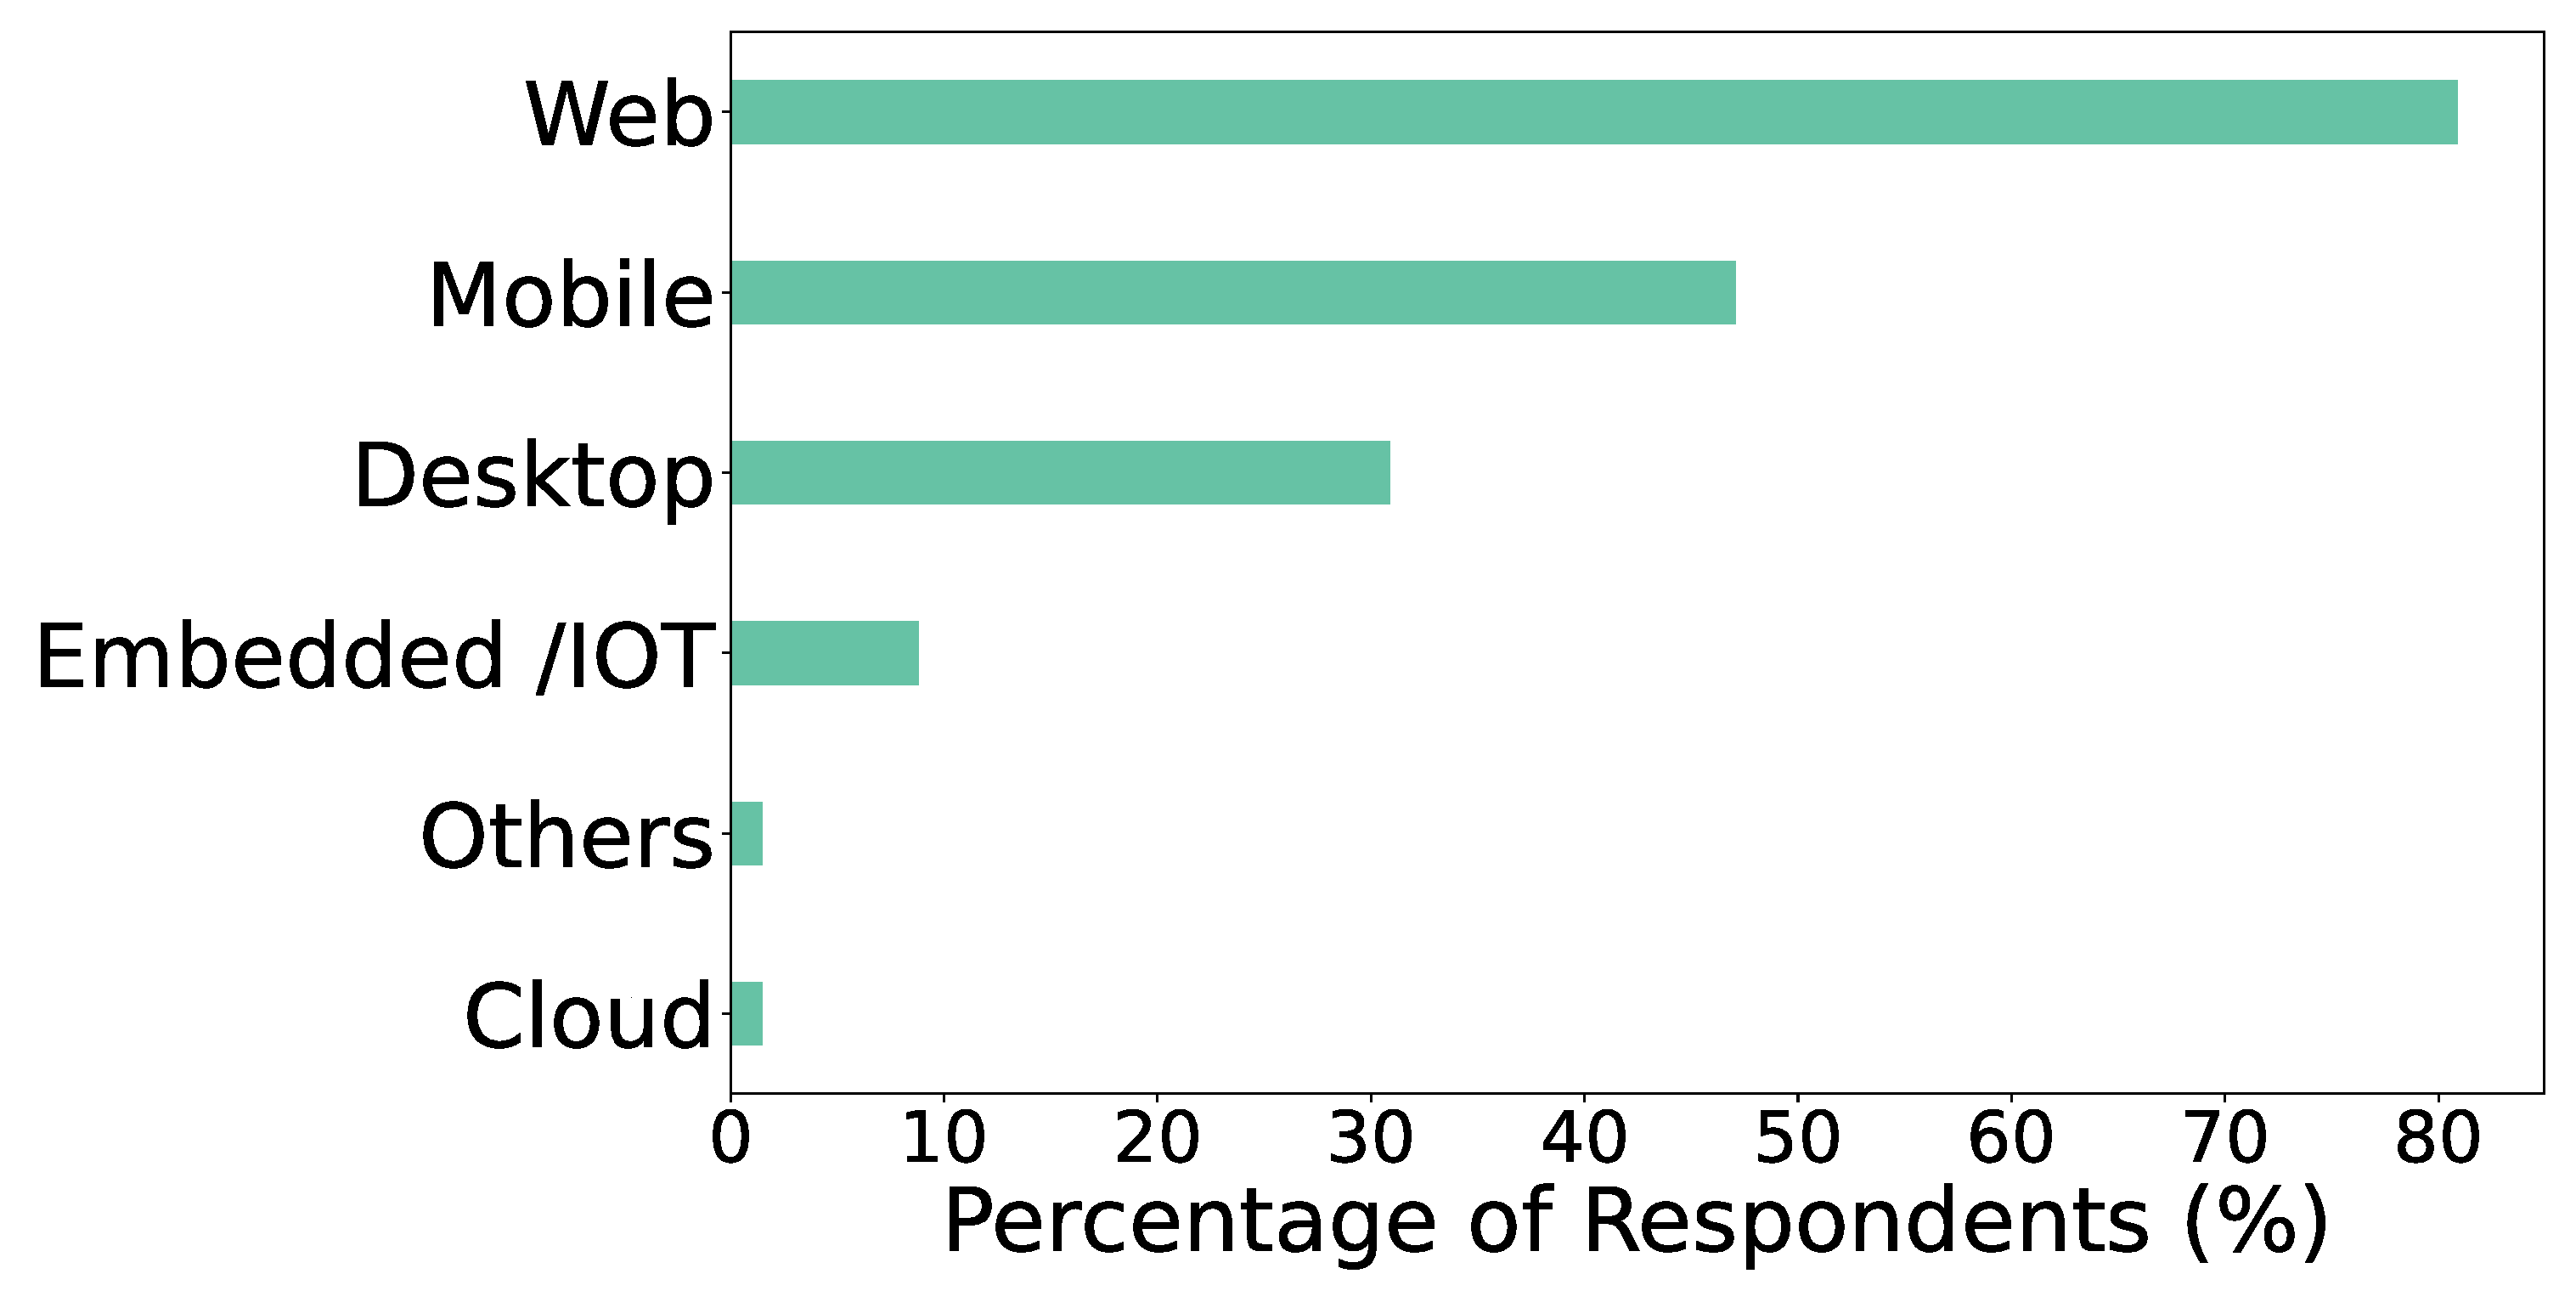
\includegraphics[scale=0.18]{Figures/Respondents_Technologies}
  \caption{Technology Platforms}
  \label{fig:platforms}
\end{figure}

\begin{figure}[h]
\centering
  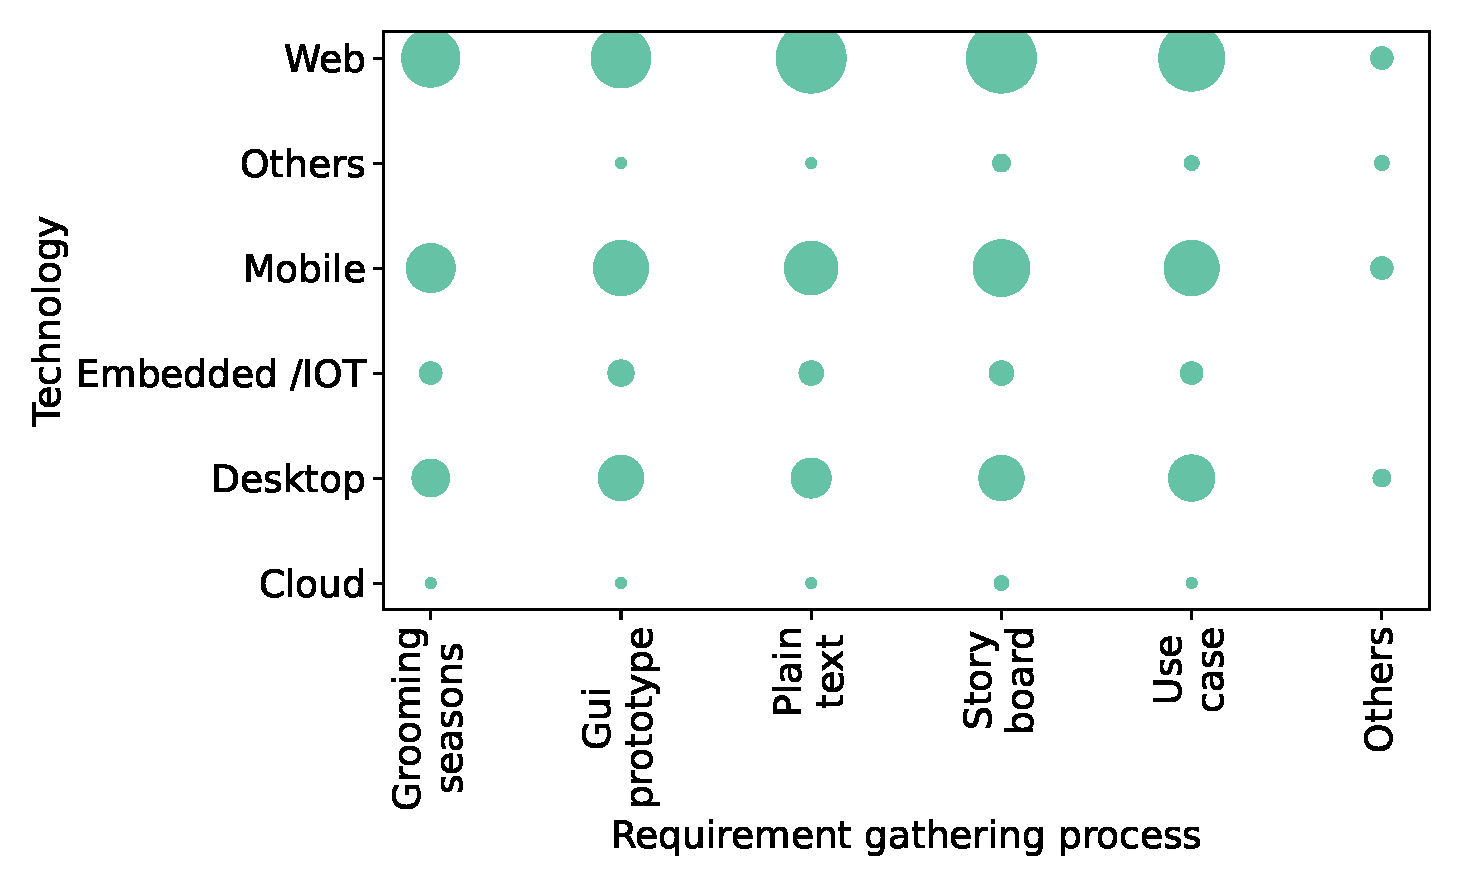
\includegraphics[scale=0.47]{Figures/Requirement_Technology_Cross_Analysis.eps}
  \caption{Cross aspect analysis of requirement gathering process and technology platform}
  \label{fig:requirement technology cross analysis}
\end{figure}

\boxtext{Web based software services have market demand in a great degree in Bangladesh.}


\paragraph{Operating Systems}
In our survey, as per Figure \ref{fig:os}, we have found that most of our respondents replied that they use Linux based operating system (56\%) as a primary operating system for their development. The second best used operating system is windows (45\%) and 28\% of the respondents use MacOS. We anticipated that the use of OS might be related to professional experience. Senior/expert developers may prefer Linux over another operating system as both usage rate of Linux among participants and participation of developers are high. We have conducted the Mann Whitney U test, and our anticipation is right (p=0.024). Senior developers prefer Linux over other operating systems.

\begin{figure}[h]
\centering
  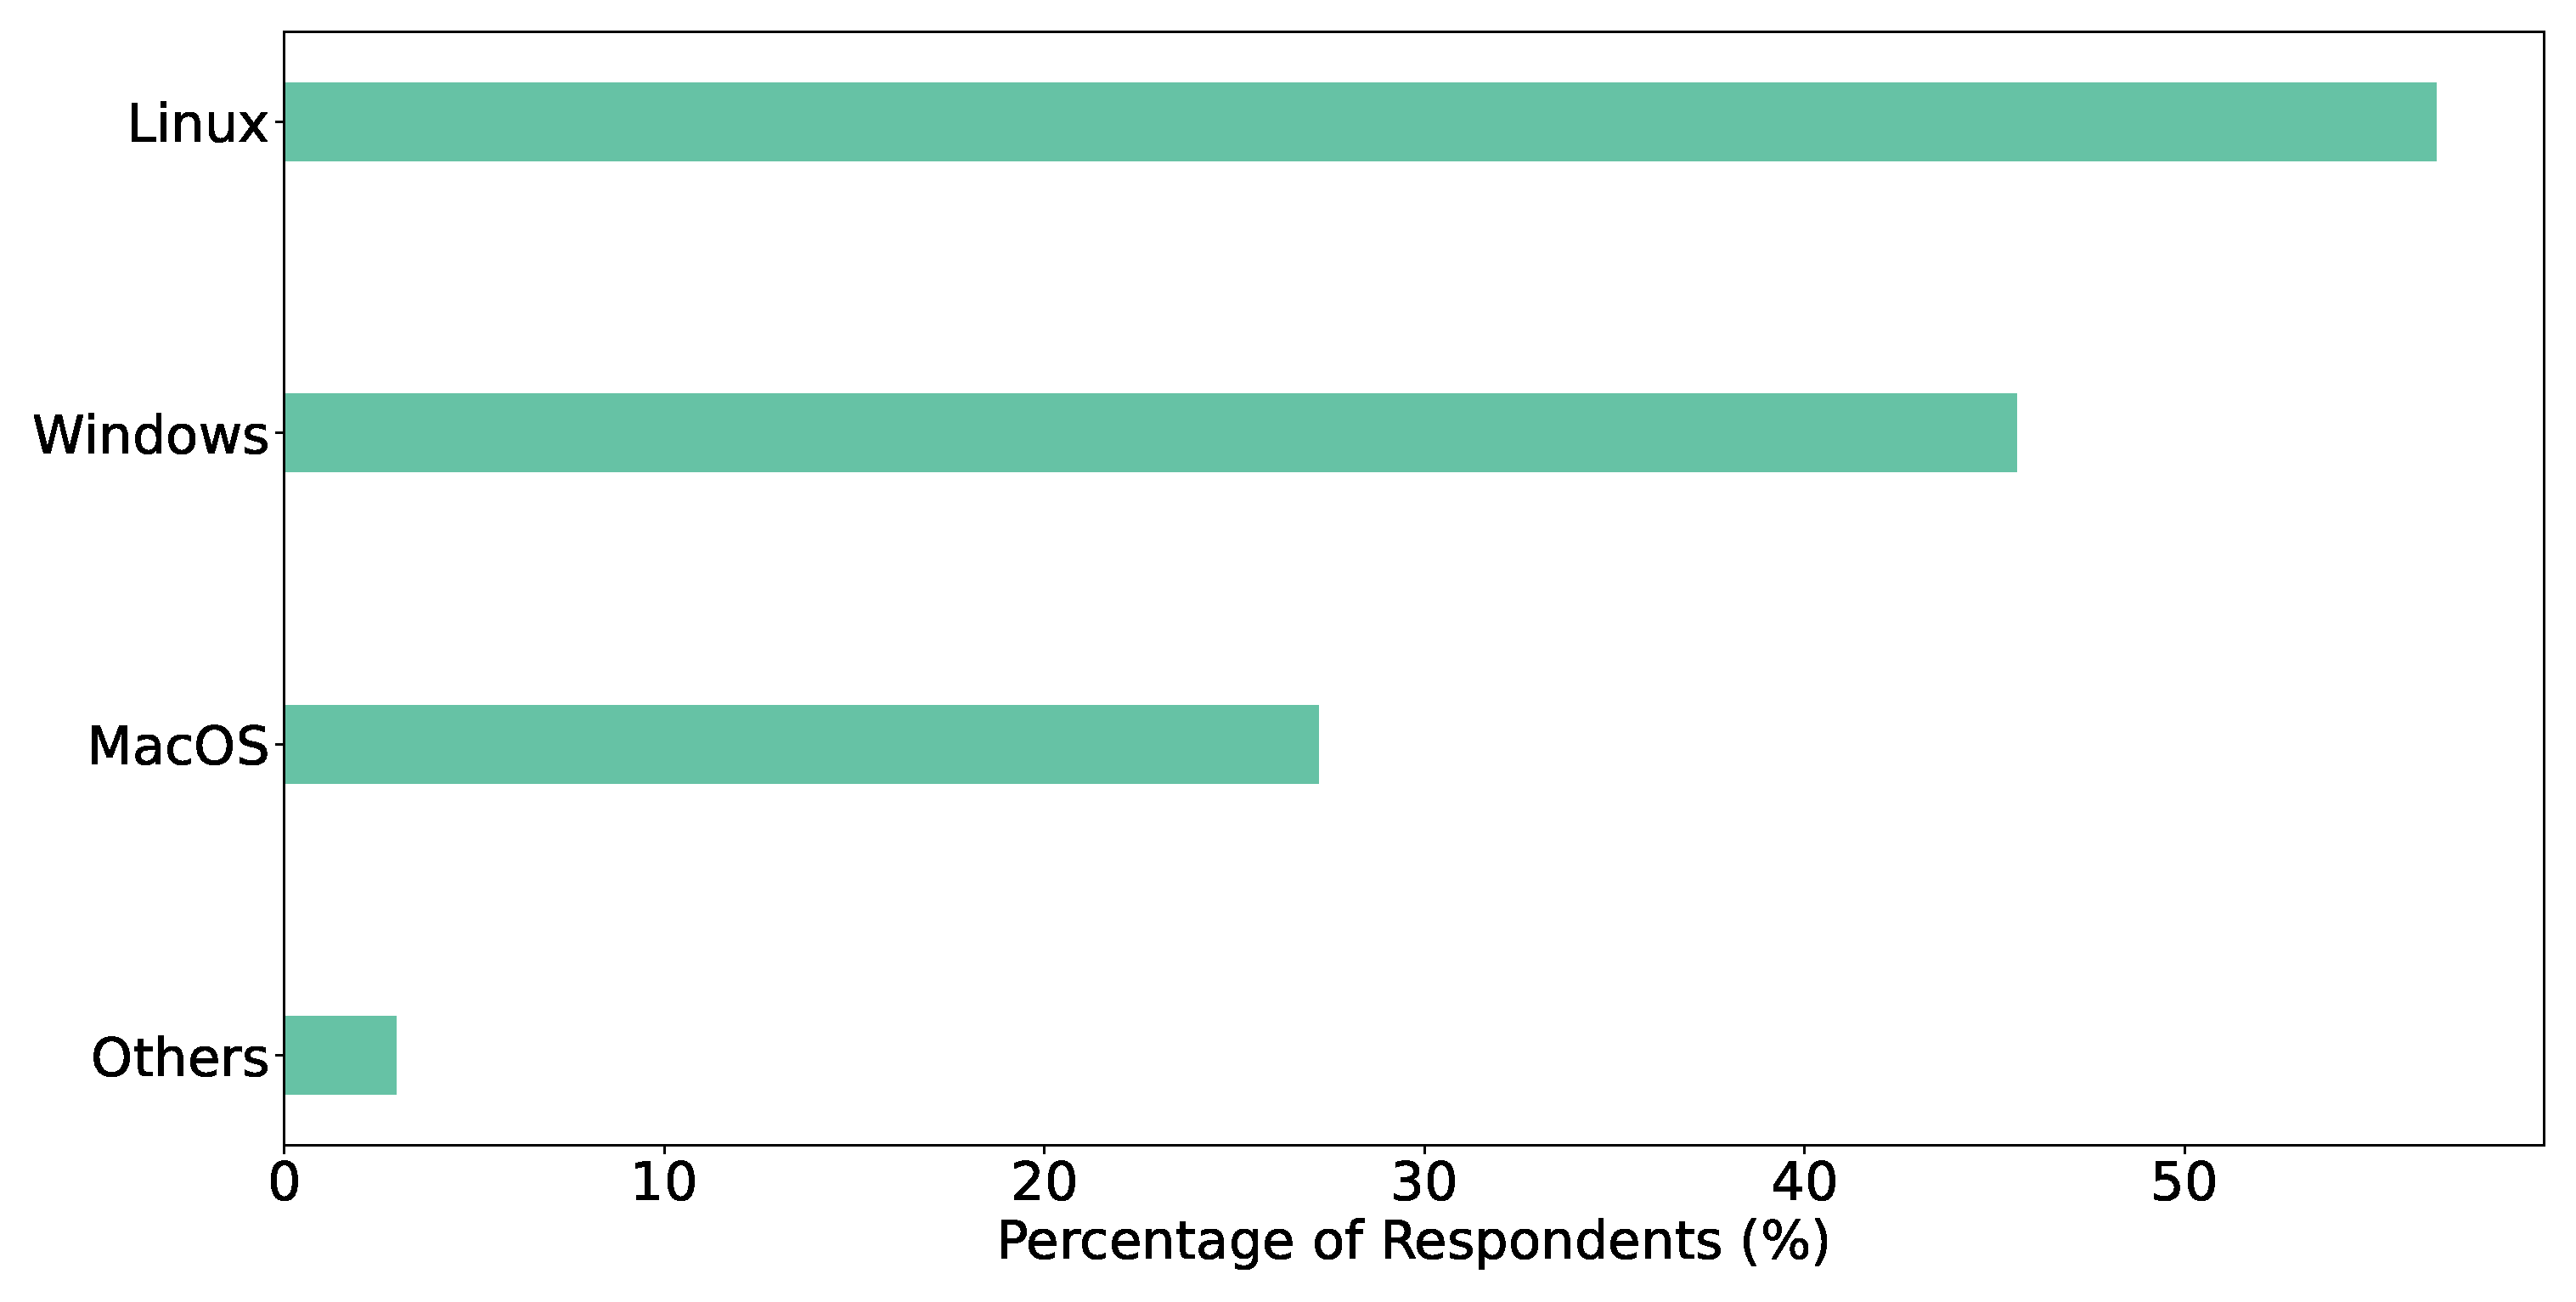
\includegraphics[scale=0.17]{Figures/Respondents_os}
  \caption{Operating Systems}
  \label{fig:os}
\end{figure}


\paragraph{Programming Languages}
According to Figure \ref{fig:languages}, around 65\% and 60\% of our respondents use Javascript and Java respectively which are two mostly used languages in Bangladesh. Other languages like php (25\%), python (25\%), c\# (18\%) are also used which indicates that the software engineers are not disposed towards a single specific language. Also the choice of programming languages used for development can have important inferences for the testing practices of a software company. We observed that users using mobile and web platforms mostly use Java and Javascript as programming languages. However, our observation is not statistically significant (p=0.1). Though the use of the operating system is influenced by programming language (e.g., Swift and macOS), we have not found any relation between the choice of programming language and operating system.
\partha{Is figure necessary for the above claim?}

\begin{figure}[h]
\centering
  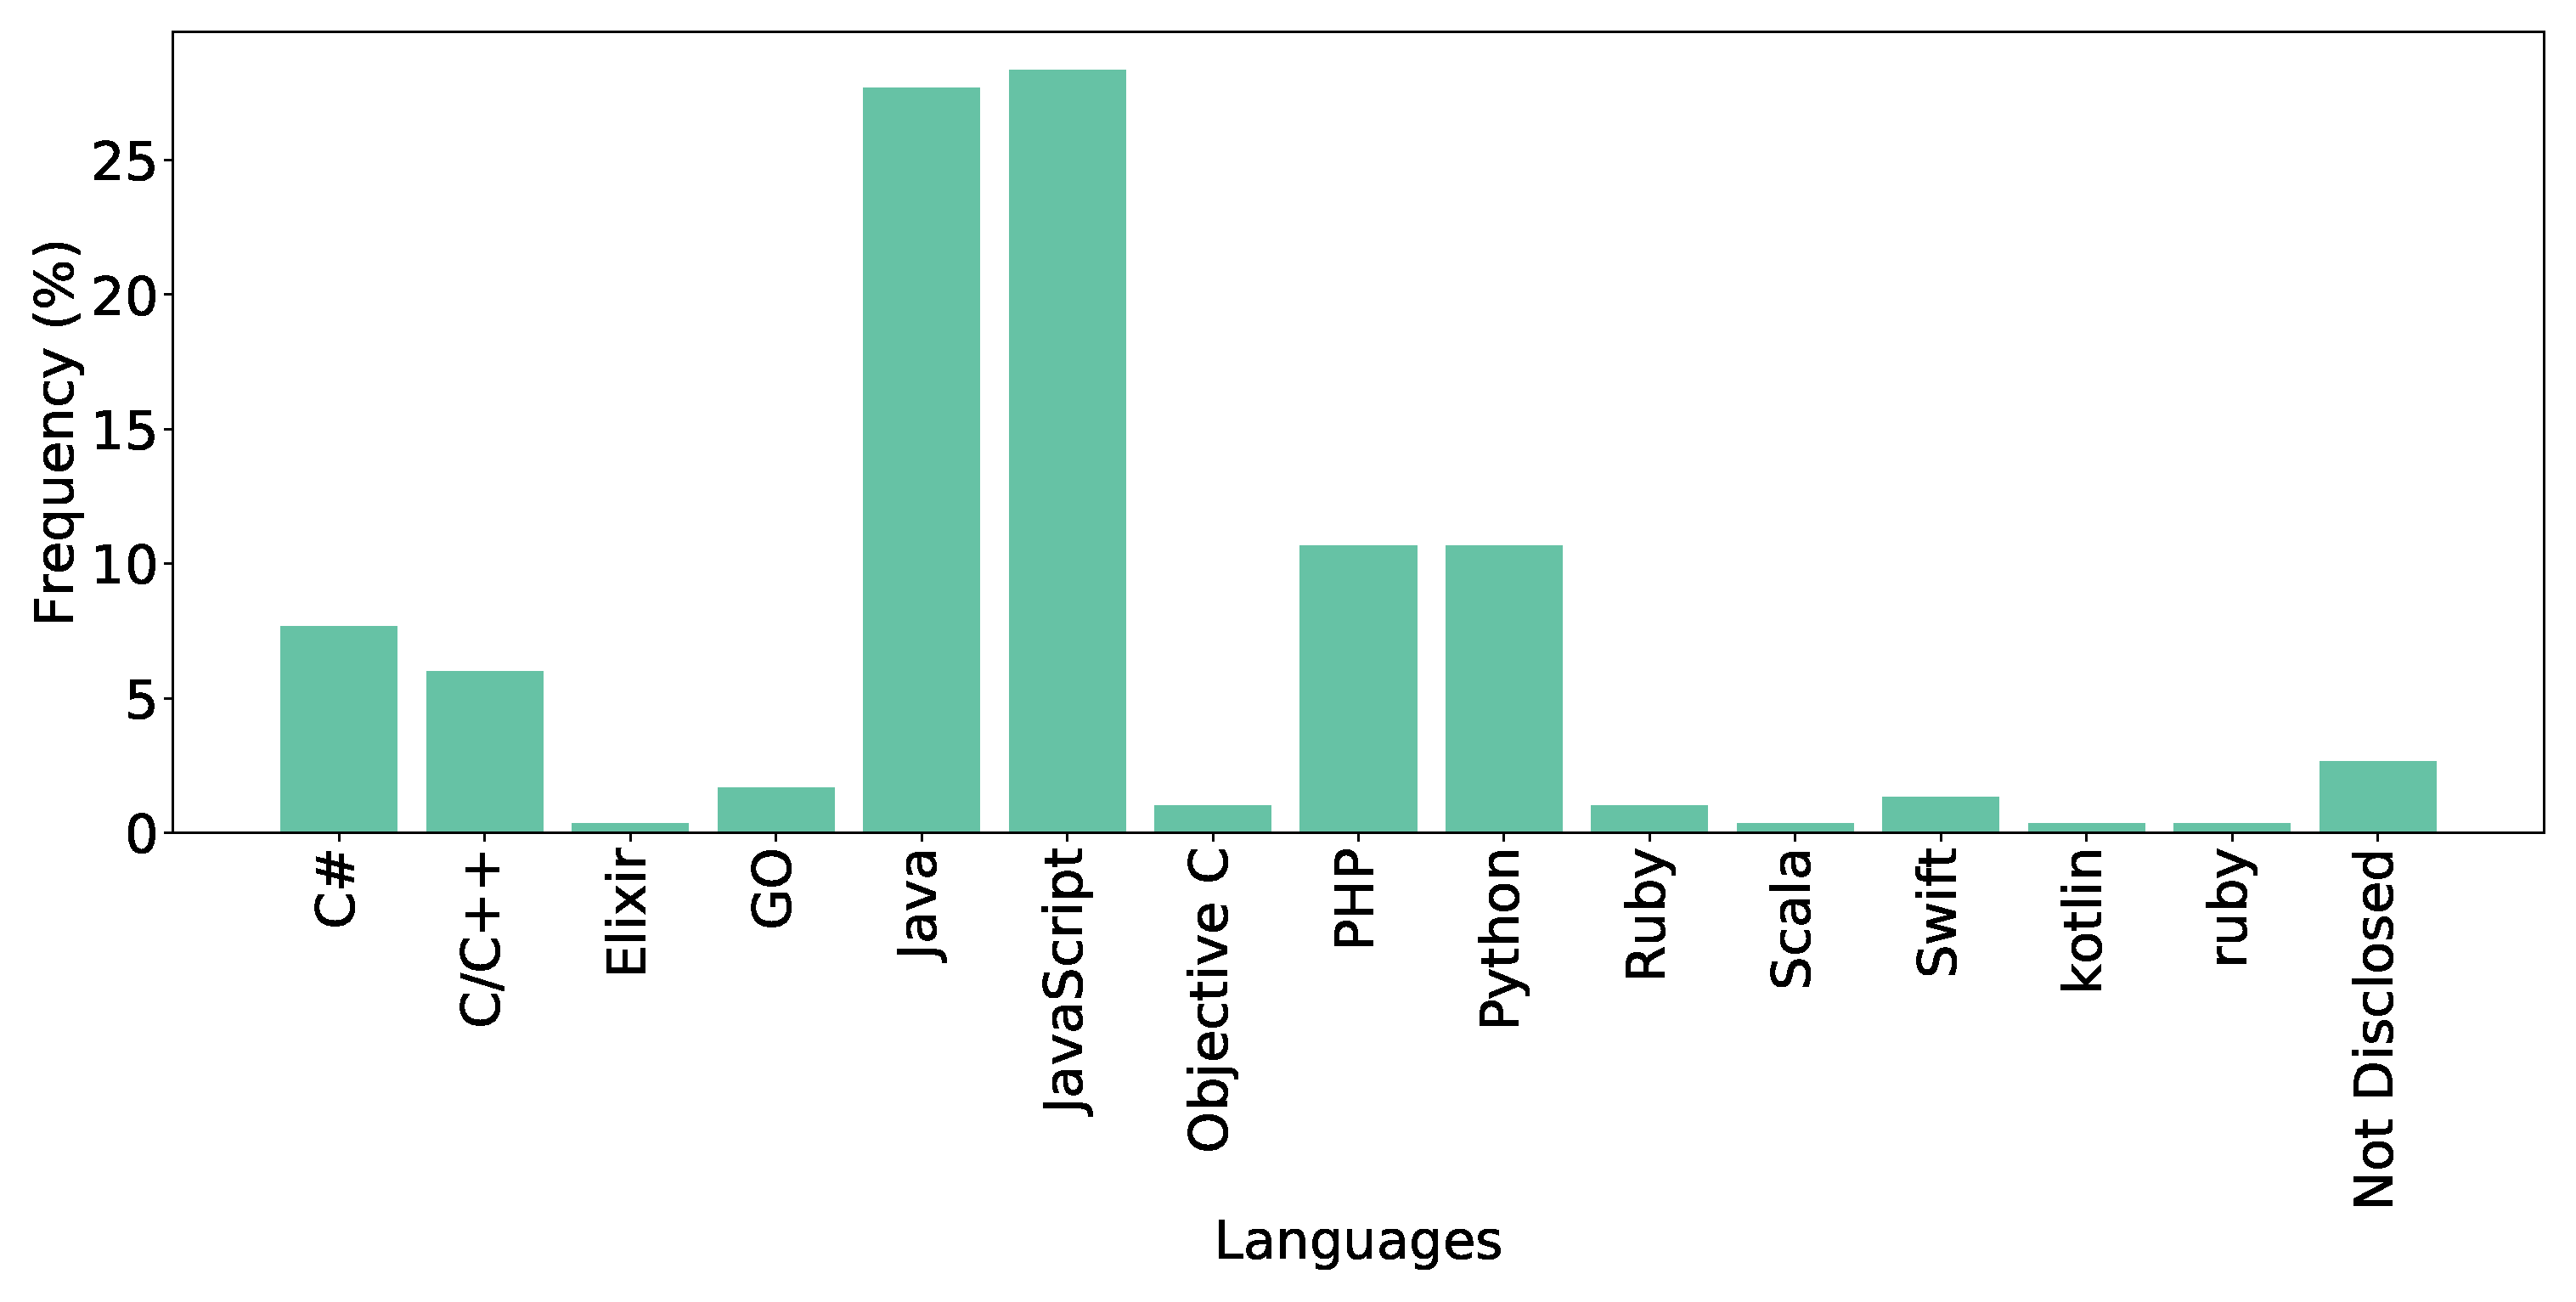
\includegraphics[scale=0.18]{Figures/Respondents_languages}
  \caption{Languages used in software development}
  \label{fig:languages}
\end{figure}

\paragraph{Frameworks used in development}
As shown in Figure \ref{fig:frameworks}, variety of frameworks have been used during development. Spring boot (37\%) is the mostly used framework in the Bangladesh's software industry which is aligned with the result of the usage rate of Java corresponding to Figure \ref{fig:languages}. Since Javascript is mostly used language of our respondents, they use various of Javascript frameworks like react, nodejs, angular, express, etc. at appreciable percentage. ASP.NET, Django and Laravel each are used in same proportion based on around 15\% of our respondents. React, Swift, Ruby on Rails, Nodejs, etc. are comparatively less used. Other than these, lot of various frameworks like Cocoa, Meteor, TestNG, Relay, Appium, CakePHP, etc. are also used in a comparatively negligible portion agglomerated in the category named others. For web development, Django and Spring frameworks are mostly used in Bangladesh (p=0.04).

\begin{figure}[h]
\centering
  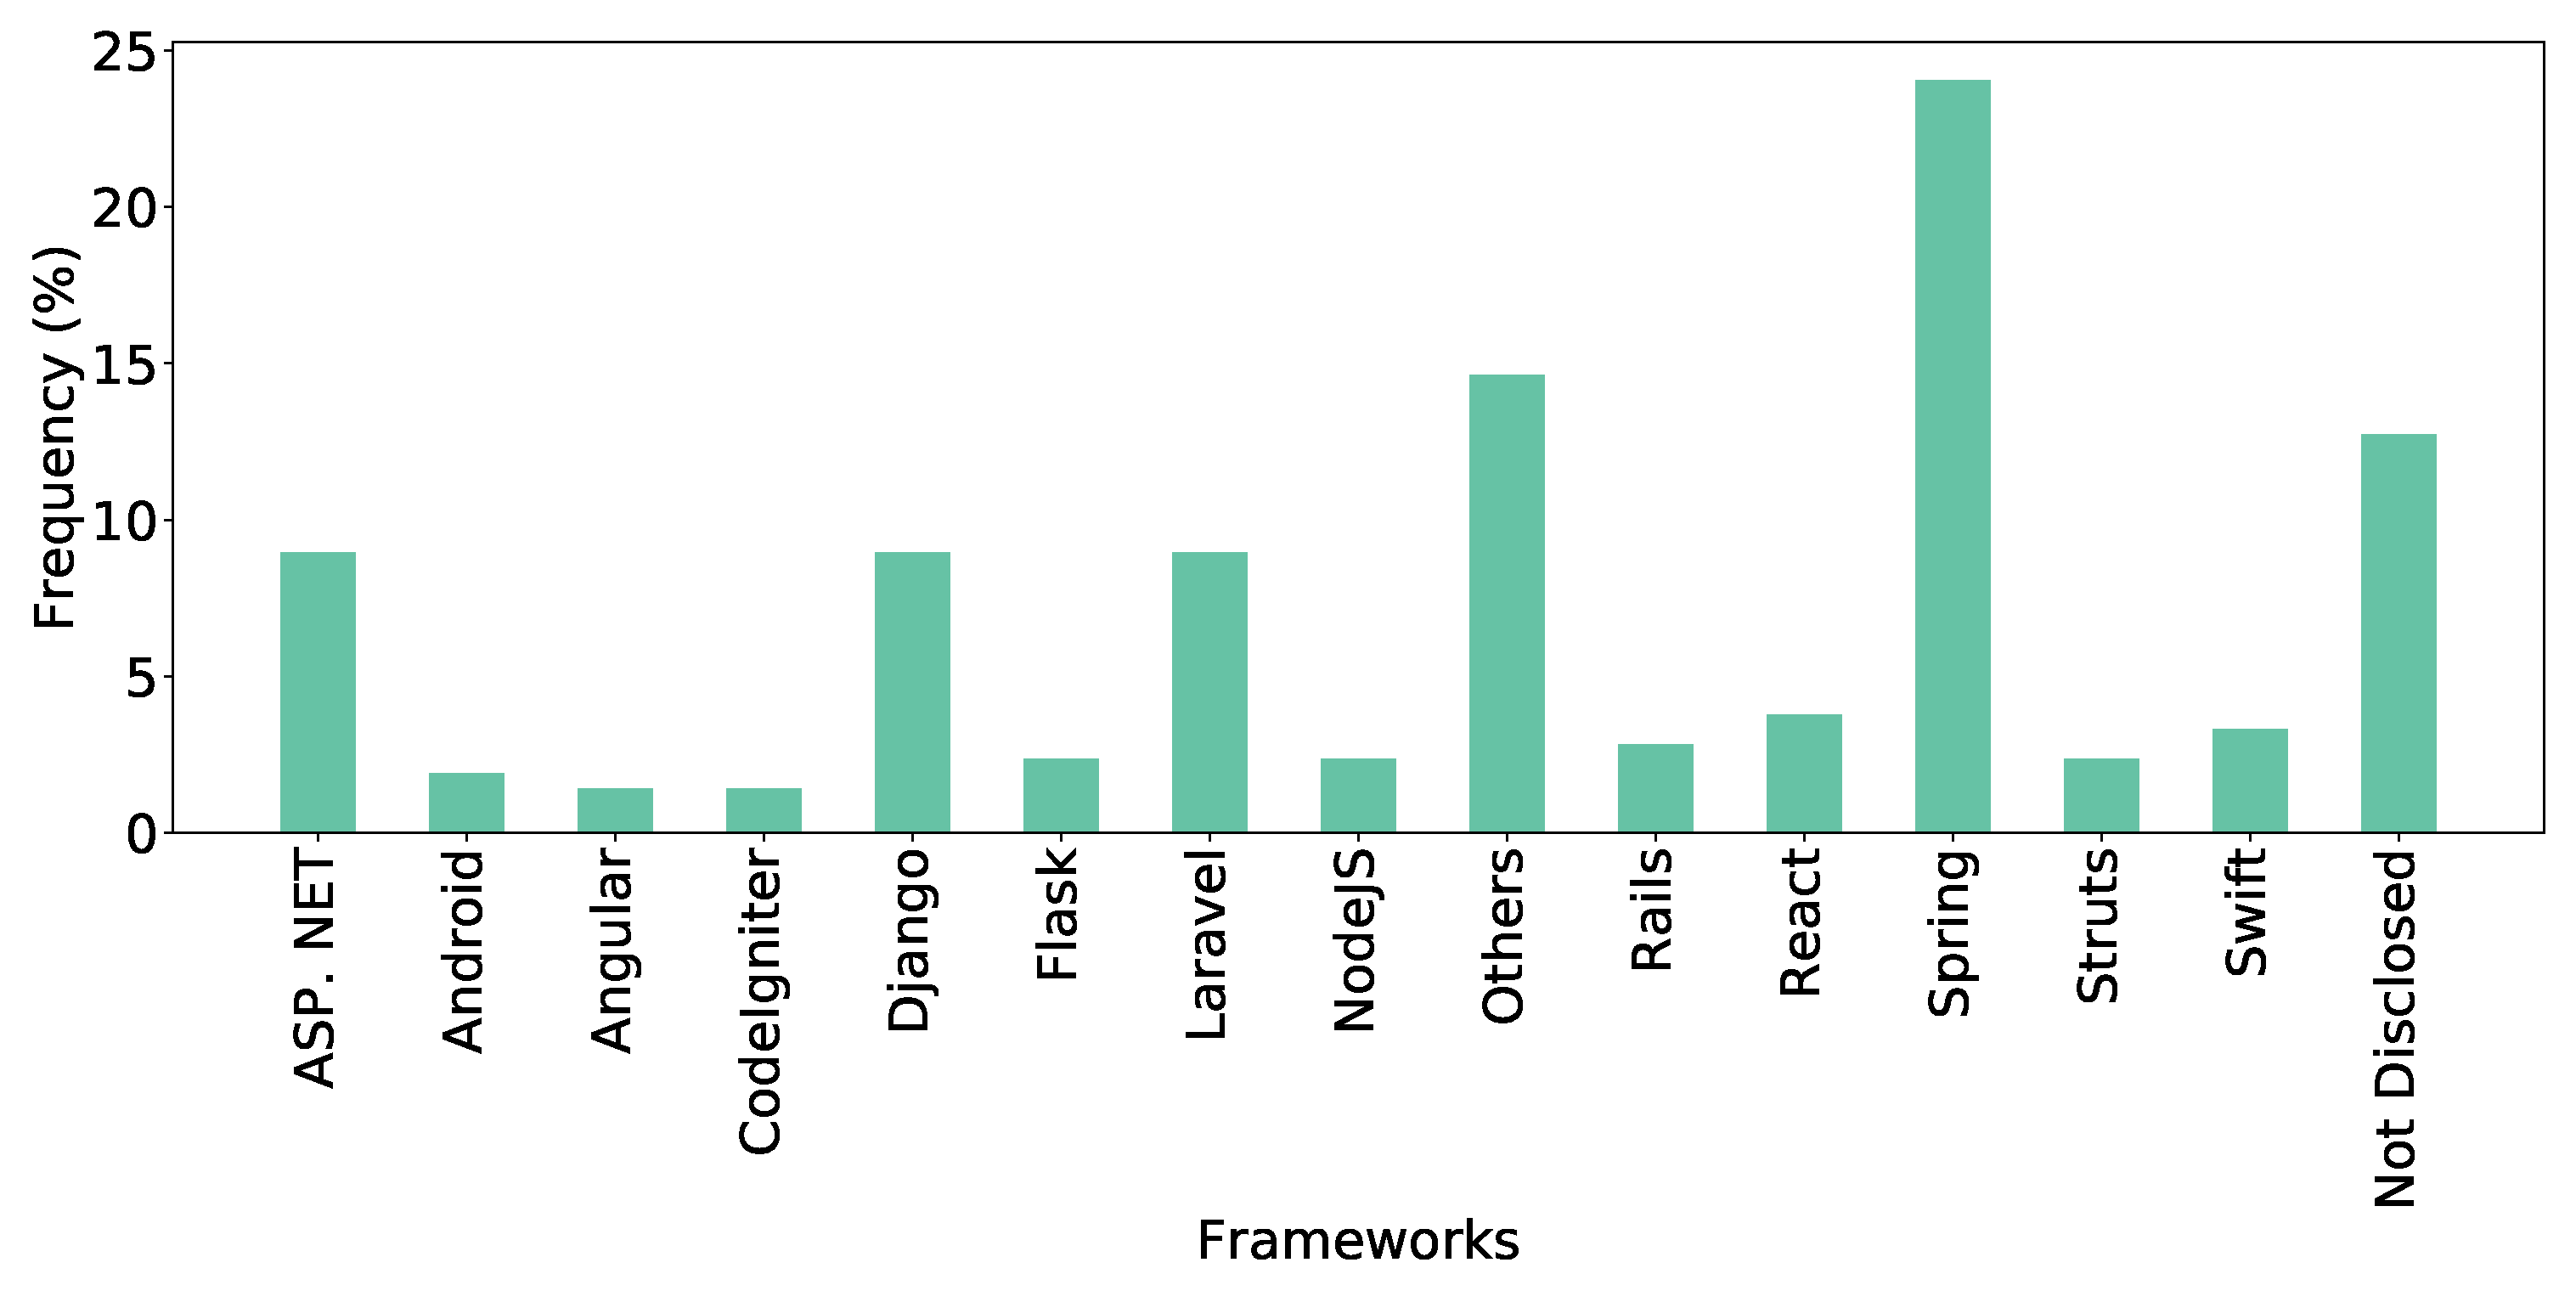
\includegraphics[scale=0.18]{Figures/Respondents_frameworks}
  \caption{Frameworks}
  \label{fig:frameworks}
\end{figure}


\paragraph{IDE's used by the respondent's}
According to Figure \ref{fig:IDEs}, IntelliJ, a Java integrated development environment for developing computer software for enterprise, mobile, and web development used by most of the respondents (43\%). The other IDEs used in SE industries are: visual studio (30\%), Eclipse (24\%), PyCharm (17\%), NetBeans (11\%), Android Studio (7\%).

\begin{figure}[htbp]
\centering
  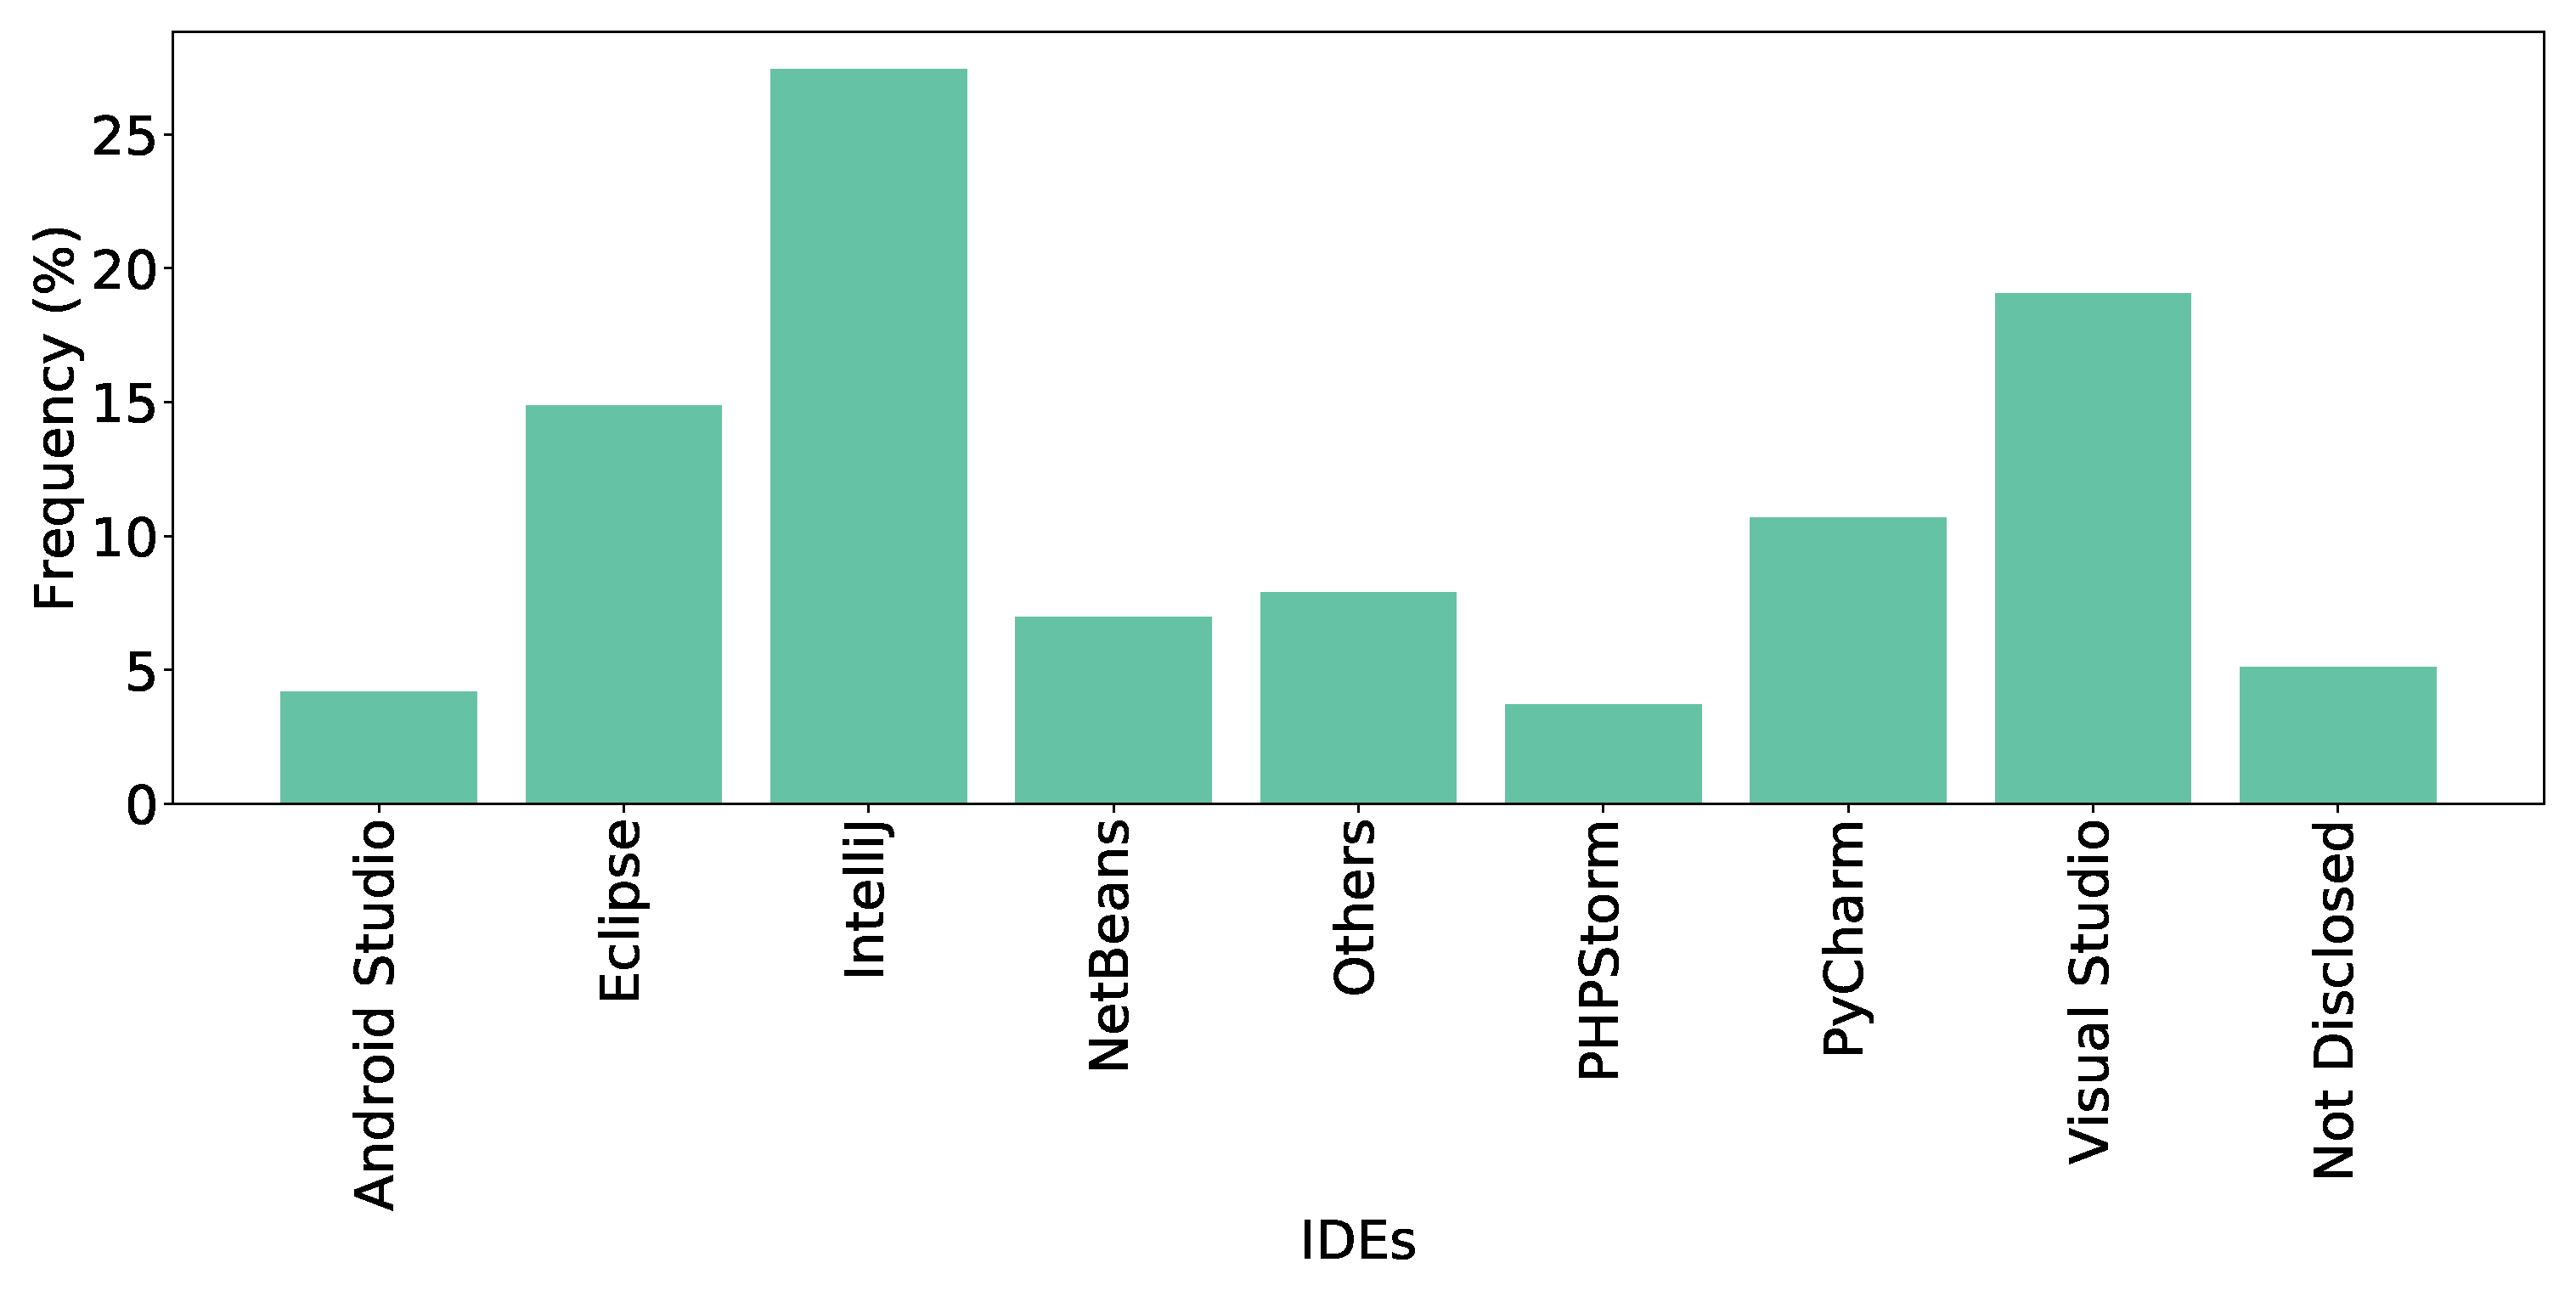
\includegraphics[scale=0.18]{Figures/Respondents_IDEs}
  \caption{IDE's}
  \label{fig:IDEs}
\end{figure}
